\documentclass{scrartcl}

\usepackage{graphicx}
\usepackage{amsmath,amssymb}
\usepackage[english]{babel}
\usepackage[utf8]{inputenc}
\usepackage{url}
\PassOptionsToPackage{hyphens}{url}\usepackage{hyperref}

\begin{document}

\section{Overview}

\begin{figure}
\centering
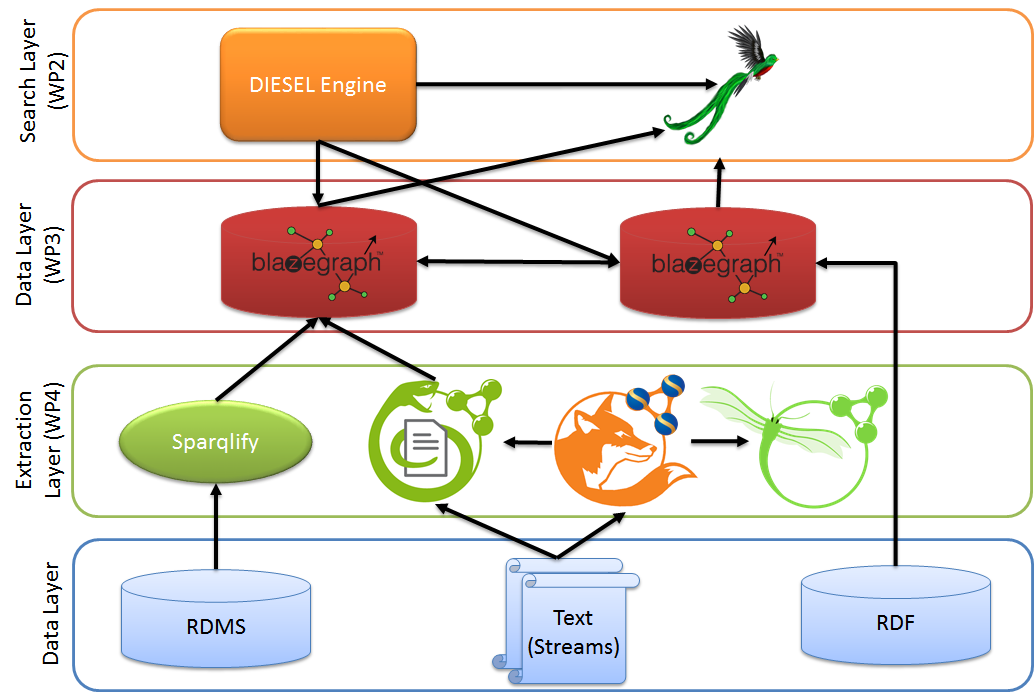
\includegraphics[width=\textwidth,keepaspectratio]{architecture.png}
\caption{The overview over the complete Diesel system.}
\label{fig:exp1-unique-results}
\end{figure}

\section{General workflow}

\begin{itemize}
	\item Input: String query, Map$<<$int, int$>$,$<$Resource $|$ Literal, double score, Type$>>$ manualAnnotations
	\item Output: 
\end{itemize}

\begin{enumerate}
\item Segmentation
	\begin{itemize}
		\item Input: String query, $<$int, int$>$ manualAnnotatedSegments
		\item Output: $<$int, int$>$ segments
		\item Task: Tokenize the text into segments that could be linked. The positions of the manual annotations are used to keep these annotations in one single segment. \textbf{Question} It might be reasonable to create more than one single segmentation and use the best of them for linking.
	\end{itemize}
\item Linking
	\begin{itemize}
		\item Input: $<$int, int$>$ segments
		\item Output: Map$<<$int, int$>$,$<$Resource $|$ Literal, double score, Type$>>$ automaticAnnotations
		\item Task: Search for Resources and Literals inside the given segments.
	\end{itemize}
\item Path Selection
	\begin{itemize}
		\item Input: Node nodes$[]$
		\item Output: List$<$List$<$Node$>>$ kShortestPaths
		\item Task:
	\end{itemize}
\item Generation
	\begin{itemize}
		\item Input: List$<$List$<$Node$>>$ kShortestPaths
		\item Output: 
		\item Task:
	\end{itemize}
\end{enumerate}

Clarify architecture/ existing modules
QUETSAL as REST

1) setup of data summaries : 
input: set<URL for SPARQL endpoints>

2) update data summary:
 input: URL or set<URL>

3) sparql endpoints via federation: 
input <SPARQL query as ?>
output result set from Jena or OpenRDF/SESAME

FOX REST + RE
input: text
output: RDF

SPARQLIFY
describe configuring process

\section{Communication between modules}

TODO discuss which are the advantages and disadvantages of the different communication styles.

\subsection{REST services}

\subsection{Micro services}

\subsection{Java monolith}



\section{Licensing}

Throughout the project the AKSW follows a dual licensing described in the following license text.

\begin{quotation}
LICENSE
This framework is provided under a dual license. For non-commercial purposes, the terms of the LGPL3.0 license hold. These terms are available at \url{http://www.gnu.org/licenses/lgpl-3.0.txt} \newline 
For commercial purposes, please contact the financial department of AKSW at jaenicke@uni-leipzig.de
\end{quotation}
\end{document}
